\documentclass{article}
\usepackage{spconf}
\usepackage{amsmath,amssymb,booktabs,cite,graphicx,microtype,url}
\setlength{\lightrulewidth}{0.6pt}\setlength{\heavyrulewidth}{0.8pt}
\urlstyle{same}
\setcounter{dbltopnumber}{1}
\setcounter{topnumber}{1}
\setcounter{totalnumber}{1}
\raggedbottom

\newcommand{\ChartCount}{1023}
\newcommand{\TitleCount}{1019}
\newcommand{\CapEightCount}{699}
\newcommand{\TopcodedGain}{+0.092}
\newcommand{\TopcodedGainLow}{+0.058}
\newcommand{\TopcodedGainHigh}{+0.127}
\newcommand{\TopcodedCapSevenGain}{+0.229}
\newcommand{\TopcodedCapSevenGainLow}{+0.182}
\newcommand{\TopcodedCapSevenGainHigh}{+0.277}
\newcommand{\TopcodedCapNineGain}{+0.044}
\newcommand{\TopcodedCapNineGainLow}{+0.014}
\newcommand{\TopcodedCapNineGainHigh}{+0.074}
\newcommand{\GbdtNativeRho}{0.897}
\newcommand{\GbdtCapEightRho}{0.435}
\newcommand{\GbdtCapEightTau}{0.338}
\newcommand{\GbdtCapEightPair}{0.709}
\newcommand{\OrdinalNativeRho}{0.890}
\newcommand{\OrdinalCapEightRho}{0.766}
\newcommand{\OrdinalCapEightTau}{0.629}
\newcommand{\OrdinalCapEightPair}{0.889}
\newcommand{\CapEightPairCount}{159,318}
\newcommand{\DojoPlacementCount}{47}
\newcommand{\DojoYearCount}{6}
\newcommand{\DojoTierCount}{5}
\newcommand{\DojoPairCount}{152}
\newcommand{\DojoRho}{0.615}
\newcommand{\DojoRhoLow}{0.248}
\newcommand{\DojoRhoHigh}{0.827}
\newcommand{\DojoPair}{0.767}
\newcommand{\DojoPairLow}{0.605}
\newcommand{\DojoPairHigh}{0.895}
\newcommand{\DojoControlPlacementCount}{201}
\newcommand{\DojoBelowCeilingPairCount}{425}
\newcommand{\DojoBelowCeilingPair}{0.626}
\newcommand{\SeqCapEightOrdinaryRho}{0.454}
\newcommand{\SeqCapEightTopcodedRho}{0.671}
\newcommand{\SeqCapEightOrdinalRho}{0.718}
\newcommand{\SeqCapEightTopcodedGain}{+0.217}
\newcommand{\SeqCapEightTopcodedGainLow}{+0.180}
\newcommand{\SeqCapEightTopcodedGainHigh}{+0.257}
\newcommand{\SeqRepresentationGain}{-0.043}
\newcommand{\SeqRepresentationGainLow}{-0.080}
\newcommand{\SeqRepresentationGainHigh}{-0.006}
\newcommand{\GlobalOrdinalLogitCapEightRho}{0.761}
\newcommand{\SeqRepresentationInterpretation}{The sequence model does not outperform global cumulative logit.}
\newcommand{\SeqDojoRho}{0.504}
\newcommand{\SeqDojoRhoLow}{0.101}
\newcommand{\SeqDojoRhoHigh}{0.756}
\newcommand{\SeqDojoPair}{0.709}
\newcommand{\SeqDojoPairLow}{0.532}
\newcommand{\SeqDojoPairHigh}{0.859}

% Generated by scripts/research/analyze_ceiling_compression.py; do not edit.
% Cap 8, capped group = charts originally rated 8--10; near cap = |output - 8| <= 0.05.
% CIs: 95% paired title-cluster bootstrap. Pct = percent of the 699 capped charts;
% Above = output > 8.05. Near-cap rho omitted when fewer than 30 near-cap charts.
\newcommand{\CeilDelta}{0.05}
\newcommand{\CeilGbdtNearPct}{56}
\newcommand{\CeilGbdtNearPctLow}{52}
\newcommand{\CeilGbdtNearPctHigh}{60}
\newcommand{\CeilGbdtNearCount}{390}
\newcommand{\CeilGbdtAbovePct}{6}
\newcommand{\CeilGbdtNearRho}{0.028}
\newcommand{\CeilGbdtNearRhoLow}{-0.075}
\newcommand{\CeilGbdtNearRhoHigh}{0.129}
\newcommand{\CeilHuberNearPct}{16}
\newcommand{\CeilHuberNearPctLow}{13}
\newcommand{\CeilHuberNearPctHigh}{19}
\newcommand{\CeilHuberNearCount}{113}
\newcommand{\CeilHuberAbovePct}{25}
\newcommand{\CeilHuberNearRho}{0.008}
\newcommand{\CeilHuberNearRhoLow}{-0.172}
\newcommand{\CeilHuberNearRhoHigh}{0.184}
\newcommand{\CeilRidgeNearPct}{12}
\newcommand{\CeilRidgeNearPctLow}{9}
\newcommand{\CeilRidgeNearPctHigh}{14}
\newcommand{\CeilRidgeNearCount}{81}
\newcommand{\CeilRidgeAbovePct}{29}
\newcommand{\CeilRidgeNearRho}{-0.164}
\newcommand{\CeilRidgeNearRhoLow}{-0.365}
\newcommand{\CeilRidgeNearRhoHigh}{0.046}
\newcommand{\CeilOneSidedNearPct}{3}
\newcommand{\CeilOneSidedNearPctLow}{2}
\newcommand{\CeilOneSidedNearPctHigh}{5}
\newcommand{\CeilOneSidedNearCount}{22}
\newcommand{\CeilOneSidedAbovePct}{80}
\newcommand{\CeilReductionNearPct}{60}
\newcommand{\CeilReductionNearPctLow}{57}
\newcommand{\CeilReductionNearPctHigh}{64}
\newcommand{\CeilReductionNearCount}{421}
\newcommand{\CeilReductionAbovePct}{0}
\newcommand{\CeilReductionNearRho}{0.683}
\newcommand{\CeilReductionNearRhoLow}{0.624}
\newcommand{\CeilReductionNearRhoHigh}{0.735}
\newcommand{\CeilSeqHuberNearPct}{19}
\newcommand{\CeilSeqHuberNearPctLow}{17}
\newcommand{\CeilSeqHuberNearPctHigh}{22}
\newcommand{\CeilSeqHuberNearCount}{136}
\newcommand{\CeilSeqHuberAbovePct}{21}
\newcommand{\CeilSeqHuberNearRho}{-0.127}
\newcommand{\CeilSeqHuberNearRhoLow}{-0.289}
\newcommand{\CeilSeqHuberNearRhoHigh}{0.038}
\newcommand{\CeilSeqOneSidedNearPct}{3}
\newcommand{\CeilSeqOneSidedNearPctLow}{2}
\newcommand{\CeilSeqOneSidedNearPctHigh}{4}
\newcommand{\CeilSeqOneSidedNearCount}{21}
\newcommand{\CeilSeqOneSidedAbovePct}{75}
\newcommand{\CeilSeqLogitNearPct}{57}
\newcommand{\CeilSeqLogitNearPctLow}{53}
\newcommand{\CeilSeqLogitNearPctHigh}{61}
\newcommand{\CeilSeqLogitNearCount}{399}
\newcommand{\CeilSeqLogitAbovePct}{0}
\newcommand{\CeilSeqLogitNearRho}{0.561}
\newcommand{\CeilSeqLogitNearRhoLow}{0.493}
\newcommand{\CeilSeqLogitNearRhoHigh}{0.625}
\newcommand{\CeilGbdtMedianEight}{7.85}
\newcommand{\CeilGbdtMedianNine}{7.99}
\newcommand{\CeilGbdtMedianTen}{8.00}
\newcommand{\CeilHuberMedianEight}{7.67}
\newcommand{\CeilHuberMedianNine}{7.96}
\newcommand{\CeilHuberMedianTen}{8.09}
\newcommand{\CeilOneSidedMedianEight}{8.26}
\newcommand{\CeilOneSidedMedianNine}{9.27}
\newcommand{\CeilOneSidedMedianTen}{10.41}


\title{Recovering Hidden Order in Saturated Difficulty Ratings}
\name{Jhen-Ke Lin}
\address{National Yang Ming Chiao Tung University\\
jacob.cs14@nycu.edu.tw}

\begin{document}
\maketitle

\begin{abstract}
Rhythm-game players choose challenges by difficulty rating, but as harder
charts join a fixed scale, many share its highest rating. A model could
provide a finer order, but must learn from tied labels that cannot confirm it.
We propose artificial top-coding, adapted from artificial censoring, which
merges known upper ratings during training to recreate the tie where the
order is known. On \textit{Taiko no Tatsujin}, gradient-boosted trees lead
seven chart-level models in full-scale correlation yet rank the merged 8--10
charts worst.
Treating the merged rating as a lower bound rather than an exact target, with
only the loss changed, improves ranking for chart-level and sequence models.
For charts actually tied at the top, lower-bound models' scores also agree
with independently designed expert-course levels. Ceiling labels should
therefore be learned as lower bounds, and rankings within them tested by
withholding known levels.
\end{abstract}

\begin{keywords}
difficulty estimation, ordinal regression, censored regression, ranking evaluation,
symbolic music
\end{keywords}

\section{Introduction}
A rhythm-game chart specifies the timed actions a player must perform.
Difficulty ratings help players choose charts, but a fixed rating scale can
lose resolution as harder content is added. In \textit{Taiko no Tatsujin},
the expert-oriented Oni chart category has an official scale from 1 to
10~\cite{bandaiSongList}. Many expert charts receive 10 even though they
appear at different stages of the game's advanced courses. This is a ceiling
effect: the highest available rating groups items that may differ in
difficulty~\cite{terwee2007ceiling}.

A model could provide a finer order for these charts, but two difficulties
arise. Its training labels are tied at the ceiling, so they give the model no
order to learn there, and the shared rating cannot establish whether a
predicted order is correct. Agreement across the full scale may mostly
reflect how well a model separates the lower levels. This resembles the range
effect in image-quality assessment, where strong correlation across a broad
range can coexist with weak discrimination within a narrow
range~\cite{li2024reqa}. At a rating ceiling, the problem is stronger: all
reference ratings in the group are identical.

Difficulty models for rhythm games and piano use chart statistics, note
sequences, and ordered
classes~\cite{tsujino2019characteristics,caronongan2021predicting,franks2023stepmania,ramoneda2022fingering}.
Franks et al.~\cite{franks2023stepmania} and Ramoneda et
al.~\cite{ramoneda2022fingering} compare predicted rankings with published
labels, player judgments, or publisher orderings. Ordinal
regression~\cite{mccullagh1980,li2006ordinal,gutierrez2016survey} and
interval-label learning~\cite{antoniuk2015interval,manwani2019pril} model
coarse labels. Closest to our test,
D\u{a}n\u{a}il\u{a} and Buiu~\cite{danaila2024censored} artificially censor
outcomes for training and validation, then score each prediction against its
original value, as PRIL~\cite{manwani2019pril} does after training on
intervals. These studies score whole-scale rankings or each censored value,
not order within a shared top rating.

Our key observation is that this tie can be recreated where the answer is known:
merging known upper levels into one rating, an operation called \emph{top
coding}, hides their order during training and model selection, while the
original ratings of held-out charts still record it. The merged rating is then
a lower bound, as in Tobit models~\cite{tobin1958}.
Motivated by this, we propose a method that makes order at the ceiling
verifiable, and use it to find how that order should be learned. Our
contributions are:
(i)~\emph{Method.} Artificial top-coding adapts artificial
censoring~\cite{danaila2024censored}: ratings 8, 9, and 10 all become 8
during training and model selection, and test scores for this \emph{capped
group} are checked against the original ratings (Sec.~\ref{sec:topcode}).
(ii)~\emph{Principle and mechanism.} Merged ratings should be learned as
lower bounds, not exact targets; an exact target pulls capped charts toward
the cap, where their order is lost (Secs.~\ref{sec:lowerbound}
and~\ref{sec:mechanism}).
(iii)~\emph{Evidence.} The model with the highest full-scale correlation
ranks the capped group worst; treating merged ratings as lower bounds
improves ranking when only the loss changes, with chart-level features and a
shared Transformer; and for the real ceiling, scores for 10-rated charts
agree with expert-course levels, an external order (Sec.~\ref{sec:results}).

\begin{figure}[t]
  \centering
  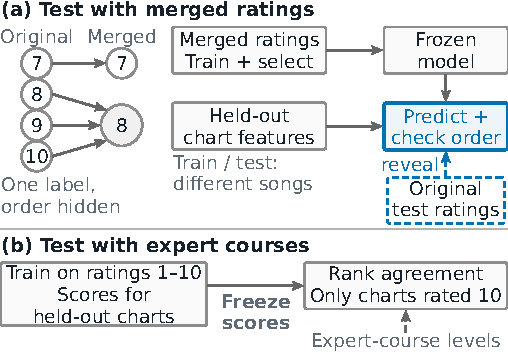
\includegraphics[width=\columnwidth]{generated/hidden_order_protocol.pdf}
  \caption{Two tests of ranking at a rating ceiling. (a) Merging known upper
  levels at a chosen cap hides their order during training and model
  selection; the original ratings of held-out charts then check the predicted
  order. (b) Separately,
  scores from models trained on the original 1--10 scale are compared with
  expert-course levels for 10-rated charts.}
  \label{fig:protocol}
\end{figure}

\section{Method}
\subsection{Artificial top-coding}
\label{sec:topcode}
For an original rating
$y_i\in\{1,\ldots,K\}$, we define the observed rating $z_i$ and the capped
group $H_c$ at the chosen cap $c$ as
\begin{equation}
 z_i=C_c(y_i)=\min(y_i,c),\qquad H_c=\{i:y_i\geq c\}.
 \label{eq:topcode}
\end{equation}
Every chart in $H_c$ has the same observed rating $c$. Permuting their original
ratings therefore leaves the observed rating vector unchanged. Any evaluation
using only that vector is invariant to the hidden permutation: it cannot
verify order within $H_c$. Chart features may still predict differences, but
checking those predictions requires information beyond the shared rating.
Artificial top-coding therefore applies Eq.~\eqref{eq:topcode} at a cap below
the real ceiling, where original ratings are known.

\begin{table*}[t]
  \centering
  \caption{Spearman correlation with original ratings. Full scale: all charts,
  after training on ratings 1--10. Cap columns: charts originally rated at
  or above the cap, after training on merged ratings; cap 8 (\CapEightCount{}
  charts) is the main comparison. Upper rows use global features; Transformer
  rows differ only in output layer and loss; each Huber pair, only in the loss.
  GBDT is highest on the full scale but lowest at caps 7 and 8.
  Brackets: SD over three seeds; other sequence results use one seed. Dashes:
  not run.}
  \label{tab:recovery}
  \begin{tabular}{lcccc}
\toprule
Model & Full scale & Cap 7 & Cap 8 & Cap 9 \\
\midrule
Huber (ordinary) & 0.881 & 0.493 & 0.640 & 0.636 \\
Huber (one-sided) & 0.883 & 0.722 & 0.732 & 0.679 \\
Ridge & 0.876 & 0.471 & 0.589 & 0.587 \\
GBDT & 0.897 & 0.349 & 0.435 & 0.599 \\
Cumulative logit & 0.878 & 0.811 & 0.761 & 0.693 \\
Cumulative probit & 0.880 & 0.809 & 0.760 & 0.690 \\
Ordinal reduction & 0.890 & 0.795 & 0.766 & 0.742 \\
\midrule
Transformer + ordinary Huber & --- & 0.415 & 0.454 {[0.033]} & 0.475 \\
Transformer + one-sided Huber & --- & --- & 0.671 {[0.010]} & --- \\
Transformer + cumulative logit & 0.885 {[0.001]} & 0.698 & 0.718 {[0.003]} & 0.701 \\
\bottomrule
\end{tabular}

\end{table*}

Figure~\ref{fig:protocol} summarizes the tests.
We split charts into five test folds by normalized song title, keeping
all versions of a song together. For each fold, the remaining charts supply
training data and a separate validation split, also grouped by title. Training,
hyperparameter selection, and early stopping use only $z_i$. Validation uses
mean absolute error (MAE) after clipping expected ratings to $[1,c]$, so
predictions above the cap are equivalent for selection. Original ratings above
the cap and course information become available only after model selection.
Each chart's \emph{test score} is an out-of-fold prediction by a model
trained without its song-title group.

We evaluate test scores $s_i$ within $H_c$ using Spearman's $\rho$, Kendall's
$\tau_b$, and \emph{pair accuracy}
\begin{equation}
 A_c=|\{(i,j)\in P_c:s_i<s_j\}|\,/\,|P_c|,
 \label{eq:pairacc}
\end{equation}
the fraction of pairs $P_c=\{(i,j):i,j\in H_c,\ y_i<y_j\}$ with unequal
original ratings that the scores order correctly. Prediction ties receive no
credit. These measures evaluate
order; score gaps are not interpreted as star units.

\subsection{Learning ceiling labels as lower bounds}
\label{sec:lowerbound}
For an artificial cap, $z_i=c$ implies $y_i\geq c$. Ordinary Huber fits
$s_i$ to $c$; one-sided Huber penalizes only $s_i<c$, as in censored
regression~\cite{tobin1958,danaila2024censored}. With Huber penalty $h_\delta$,
\begin{equation}
 \ell_{\mathrm{1s}}(s,z;c)=
 \begin{cases}
   h_\delta(s-z),&z<c,\\
   \phi(c-s),&z=c.
 \end{cases}
 \label{eq:onesided}
\end{equation}
The global solver uses $\phi(u)=\max(u,0)$; the Transformer uses
$\phi(u)=h_\delta(\max(u,0))$. Both penalties are zero when $s\geq c$; on
the original scale, $c=10$. For $z<c$, Eq.~\eqref{eq:onesided} equals the
ordinary Huber loss, so the two differ only on capped charts.
Ordinal models are instances of the same principle. Cumulative logit and
probit models place ordered thresholds on a latent
score~\cite{mccullagh1980}; they and ordinal reduction into nested binary
classification tasks impose no upper target on capped charts.

An exact target pulls
predictions for capped charts toward $c$; the loss treats any spread among
capped charts as error, so order within the ceiling is flattened. A lower
bound does not penalize predictions above $c$, and ordinal likelihoods keep
rewarding confidence in the top level, so charts whose features indicate
greater difficulty still score higher, and order is preserved.

\section{Experimental Setup}
\subsection{Data and representations}
We use \ChartCount{} unique Oni charts from \TitleCount{} song-title groups.
Each chart contains drum-action types and timings, tempo, scroll speed, and
sustained actions. These symbolic event sequences provide both chart-level
summary features, called \emph{global features} below, and inputs to a
Transformer. The 19 global features summarize duration, note density, time
between onsets, tempo, scroll speed, and note types. The sequence model
encodes drum-action type, onset within the measure, sustained-action duration,
tempo, scroll speed, and nearby events per second. Two- and four-measure
windows start every two measures, with at most 128 events per window and 64
windows per chart.

\subsection{Models and training}
We compare seven global models: ordinary Huber regression, one-sided Huber
regression, ridge regression, gradient-boosted decision trees (GBDT),
cumulative logit and probit models, and ordinal reduction. Ordinary Huber,
ridge, and GBDT fit the cap as an exact target; the others treat it as a
lower bound. All global models use the same training, validation, and test
partitions.

A four-layer, 256-dimensional
Transformer~\cite{vaswani2017attention} encodes each window; averaging valid
events and windows gives the chart representation. Ordinary Huber, one-sided
Huber, and cumulative logit share the encoder, partitions, optimizer, and
training budget; only the output layer and loss change. At cap 8, all three
sequence models use five folds and seeds 2025--2027. Caps 7 and 9 use
prespecified single-seed ordinary Huber and cumulative logit runs. The
full-scale sequence model uses cumulative logit with three seeds. After
selecting an epoch, we refit on the fold's training charts. Scores are
standardized using that training set before combining folds and seeds.
Hyperparameter grids, optimizer settings, per-seed results, and run
status are in the accompanying artifact.

Cap 8, fixed before any merged-rating result was generated, is the main
comparison; caps 7 and 9 test sensitivity to the choice of threshold.
Confidence intervals for model differences use 10,000 paired bootstrap
samples of whole song-title groups.

\subsection{Comparison with expert courses}
Dan-i Dojo is an official progression mode with increasingly advanced levels,
each prescribing a three-chart course~\cite{bandaiDaniDojo}. We use public
community-maintained transcriptions of course tables for
2020--2025~\cite{taikoWikiDani}. The official mode description does not verify
each transcribed row. Course placement was designed
independently of our model. To compare equally rated charts, the main analysis
retains only Oni charts rated 10, across 10th Dan, Kuroto, Meijin, Chojin, and
Tatsujin, in increasing course level.

For this test, global one-sided Huber and sequence cumulative logit models,
both of which learn the top rating as a lower bound, are trained on the
original 1--10 scale. We freeze their
test scores before matching chart and course records by exact normalized
title. Ambiguous or unmatched titles are excluded. This yields
\DojoPlacementCount{} placements across \DojoYearCount{} editions and
\DojoTierCount{} course levels. We compute Spearman correlation and pair
accuracy within each year, comparing pairs from different course levels, then
average the yearly values with equal weight. A 10,000-sample bootstrap resamples years, then placements within each
year. A permutation test shuffles course levels within each year.
As a control, we compare equally rated charts below 10. Position within a
three-chart course is exploratory: only four main-analysis courses match all
three positions, and position need not imply difficulty order.

\section{Results}
\label{sec:results}
\subsection{Ranking after merging ratings}
\label{sec:reversal}
Table~\ref{tab:recovery} shows that full-scale correlation and ranking within
the capped group favor different models. Among seven global models, GBDT has the
highest full-scale correlation ($\rho=\GbdtNativeRho$) but the lowest cap-8
correlation ($\GbdtCapEightRho$). Ordinal reduction is second on the full
scale ($\OrdinalNativeRho$) and first at cap 8 ($\OrdinalCapEightRho$),
evaluated on the same \CapEightCount{} charts.
The reversal also appears in Kendall correlation and pair accuracy. On the
\CapEightPairCount{} unequal-rating pairs at cap 8, GBDT gives
$\tau_b=\GbdtCapEightTau$ and $A_8=\GbdtCapEightPair$; ordinal reduction gives
$\OrdinalCapEightTau$ and $\OrdinalCapEightPair$, respectively.

\begin{figure}[t]
  \centering
  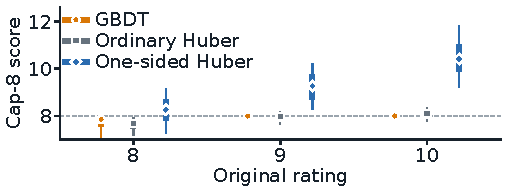
\includegraphics[width=\columnwidth]{generated/ceiling_compression.pdf}
  \caption{Test scores of the \CapEightCount{} capped-group charts at cap 8
  by original rating, for three global models trained on merged ratings.
  Markers: medians; thick bars: middle 50\%; thin bars: 10th--90th
  percentiles. Dashed line: the cap.}
  \label{fig:mechanism}
\end{figure}

\subsection{Mechanism of the reversal}
\label{sec:mechanism}
Figure~\ref{fig:mechanism} shows where capped-group scores fall relative to
the cap. GBDT places \CeilGbdtNearPct\% of capped-group test
scores within \CeilDelta{} of the cap, and within this band their Spearman
correlation with original ratings is \CeilGbdtNearRho{} (95\% CI
[\CeilGbdtNearRhoLow, \CeilGbdtNearRhoHigh]). Ordinary Huber
places fewer scores there (\CeilHuberNearPct\%), but they are likewise
unordered ($\rho=\CeilHuberNearRho$ [\CeilHuberNearRhoLow, \CeilHuberNearRhoHigh]).
One-sided Huber places only
\CeilOneSidedNearPct\% near the cap, and its scores rise above the cap with original
rating. Concentration at the cap alone does not remove order: ordinal
reduction places \CeilReductionNearPct\% of its scores within \CeilDelta{} of the cap, yet
keeps them ordered ($\rho=\CeilReductionNearRho$
[\CeilReductionNearRhoLow, \CeilReductionNearRhoHigh]). Exact targets thus pull capped
charts toward the cap, where their scores carry little order; lower-bound and
ordinal models keep that order.

\subsection{Learning merged ratings as lower bounds}
\label{sec:lbresults}
For global Huber regression, treating the cap as a lower bound improves
Spearman correlation by \TopcodedGain{} (95\% CI
[\TopcodedGainLow, \TopcodedGainHigh]). Gains at caps 7 and 9 are
\TopcodedCapSevenGain{} [\TopcodedCapSevenGainLow, \TopcodedCapSevenGainHigh]
and \TopcodedCapNineGain{} [\TopcodedCapNineGainLow, \TopcodedCapNineGainHigh].
Global ordinal models, which also impose no upper target, match or exceed
the one-sided model. At
every cap, the three lowest global correlations come from models that fit the
cap as an exact target.

With the shared Transformer, ordinary Huber, one-sided Huber, and cumulative
logit reach cap-8 correlations of \SeqCapEightOrdinaryRho{},
\SeqCapEightTopcodedRho{}, and \SeqCapEightOrdinalRho{}. The one-sided gain
over ordinary Huber is \SeqCapEightTopcodedGain{} (95\% CI
[\SeqCapEightTopcodedGainLow, \SeqCapEightTopcodedGainHigh]). With only the
loss changed, the gain is attributable to the treatment of merged ratings.

Compared with global cumulative logit ($\rho=\GlobalOrdinalLogitCapEightRho$),
the sequence cumulative logit model differs in correlation by
\SeqRepresentationGain{} (95\% CI
[\SeqRepresentationGainLow, \SeqRepresentationGainHigh]). This comparison
changes both input representation and architecture, so it compares complete
systems without isolating the effect of temporal information.
\SeqRepresentationInterpretation{} A larger corpus could change this ranking.

\begin{figure}[t]
  \centering
  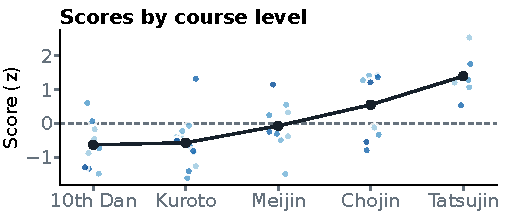
\includegraphics[width=\columnwidth]{generated/dojo_criterion.pdf}
  \caption{Scores rise with course level among 10-rated charts
  (\DojoPlacementCount{} placements); models are trained on ratings 1--10.
  Global one-sided Huber scores, standardized within each year (darker blue:
  later year); black points are course-level means.}
  \label{fig:dojo}
\end{figure}

\subsection{Agreement with expert-course levels}
\label{sec:dojo}
Figure~\ref{fig:dojo} compares model scores with course levels among charts all
rated 10. Global one-sided Huber scores have mean yearly Spearman correlation
$\rho=\DojoRho$ (95\% CI [\DojoRhoLow, \DojoRhoHigh]) and mean yearly pair
accuracy \DojoPair{} [\DojoPairLow, \DojoPairHigh] from \DojoPairCount{}
eligible pairs, a mean of yearly accuracies, not a pooled fraction. Both
permutation tests give $p<.001$.

The sequence cumulative logit model agrees in direction, with mean yearly
$\rho=\SeqDojoRho$ [\SeqDojoRhoLow, \SeqDojoRhoHigh] and pair accuracy
\SeqDojoPair{} [\SeqDojoPairLow, \SeqDojoPairHigh]. In the control analysis of
\DojoControlPlacementCount{} matched Oni placements, global scores correctly
order a fraction \DojoBelowCeilingPair{} of the
\DojoBelowCeilingPairCount{} within-year pairs sharing a rating below 10.
This weaker control is descriptive because course composition and the
distribution of ratings vary across course levels.

\section{Discussion and Conclusion}
Correlation with published ratings and correct ranking within their
highest category are separate properties; GBDT's reversal shows that the
second needs its own evaluation. Comparisons across model families describe
this dataset, not a universal advantage for any estimator.

Agreement with expert courses supports using scores to suggest smaller
progression steps or flag disagreements for content review within an official
rating. The scores express relative order and are not a calibrated extension
of the star scale: a score of 13 does not mean three stars above 10. Official
ratings remain the primary labels.

Original ratings provide the evaluation order in the artificial-cap test;
they are not psychophysical ground truth. Course levels likewise reflect
design choices, including pattern coverage, novelty, and the other charts in
a course. The course comparison contains \DojoPlacementCount{} placements
across six editions; exact matching excludes three otherwise eligible
placements. The course comparison covers two models, so
the model reversal is tested only under artificial caps. The study covers one
game and one expert chart category. It evaluates recovery of rating order and
agreement with course design; it does not measure player performance or
establish generalization to other domains.

Merging known levels creates a direct test of ranking at a ceiling, and
ceiling labels should be learned as lower bounds. Applying the
procedure elsewhere requires an ordinal scale whose upper levels can be
withheld, or an external source of order; a real ceiling with neither cannot
be validated from its shared rating alone. Rankings within a shared top rating
can, and should, be evaluated wherever upper levels can be withheld or an
external order exists.

\medskip
\noindent\textbf{Acknowledgments.} Anthropic Claude and OpenAI GPT
translated, edited, and revised text in all sections, supported discussion of
the content, and, as instructed by the author, wrote the experiment code and
the code for visualizations. The author verified all outputs and is responsible
for the content.

\clearpage
\section*{Compliance with Ethical Standards}
This study analyzes no human participants, player records, interactions, or
interventions; its external criterion is publicly documented course placement.
This study received no external funding, sponsorship, or donated computing
resources. The author has no conflicts of interest to disclose.

\bibliographystyle{IEEEbib}
\bibliography{references}
\end{document}
